\chapter{Method/Approach (theoretical)}
Extracting information from documents written in text is not a simple task due to the nature of the complexity of natural language. \cite{t2m_1} identified several obstacles to performing the information extraction: \textit{Syntactic Leeway} describes the problem of inconsistency between the semantic and syntactic aspects of the textual representation. \textit{Atomicity} refers to the problem of adequately mapping the phase-activities. \textit{Relevance} checks whether some part of the text input is irrelevant to the process model, such as examples offered by authors, which helps the human reader to understand the described process but introduces noise for information extraction. \textit{Referencing} deals with the question of how to identify the references between sentences, e.g., the pronouns "This" and "it", from the sentence "After this step, it will be delivered to ...".

Our model will use regulatory documents as input files. In the first step, the input file will be pre-processed. The documents will be split into sentences using tokenization. Correctly identifying the end of sentences is crucial for further information processing. Then, the words in the sentence should be tagged with a proper grammatical label so that we can analyze the relationship between words. In the pre-processing, it is also very important to identify the business process elements, such as the actors and actions. This step should also tackle the problem of active and passive voice. After all tasks in pre-processing, the tagged documents will be used for the analysis of the relationship between sentences.

\begin{figure}[h]
    \centering
    \caption{Overview of pre-processing}
    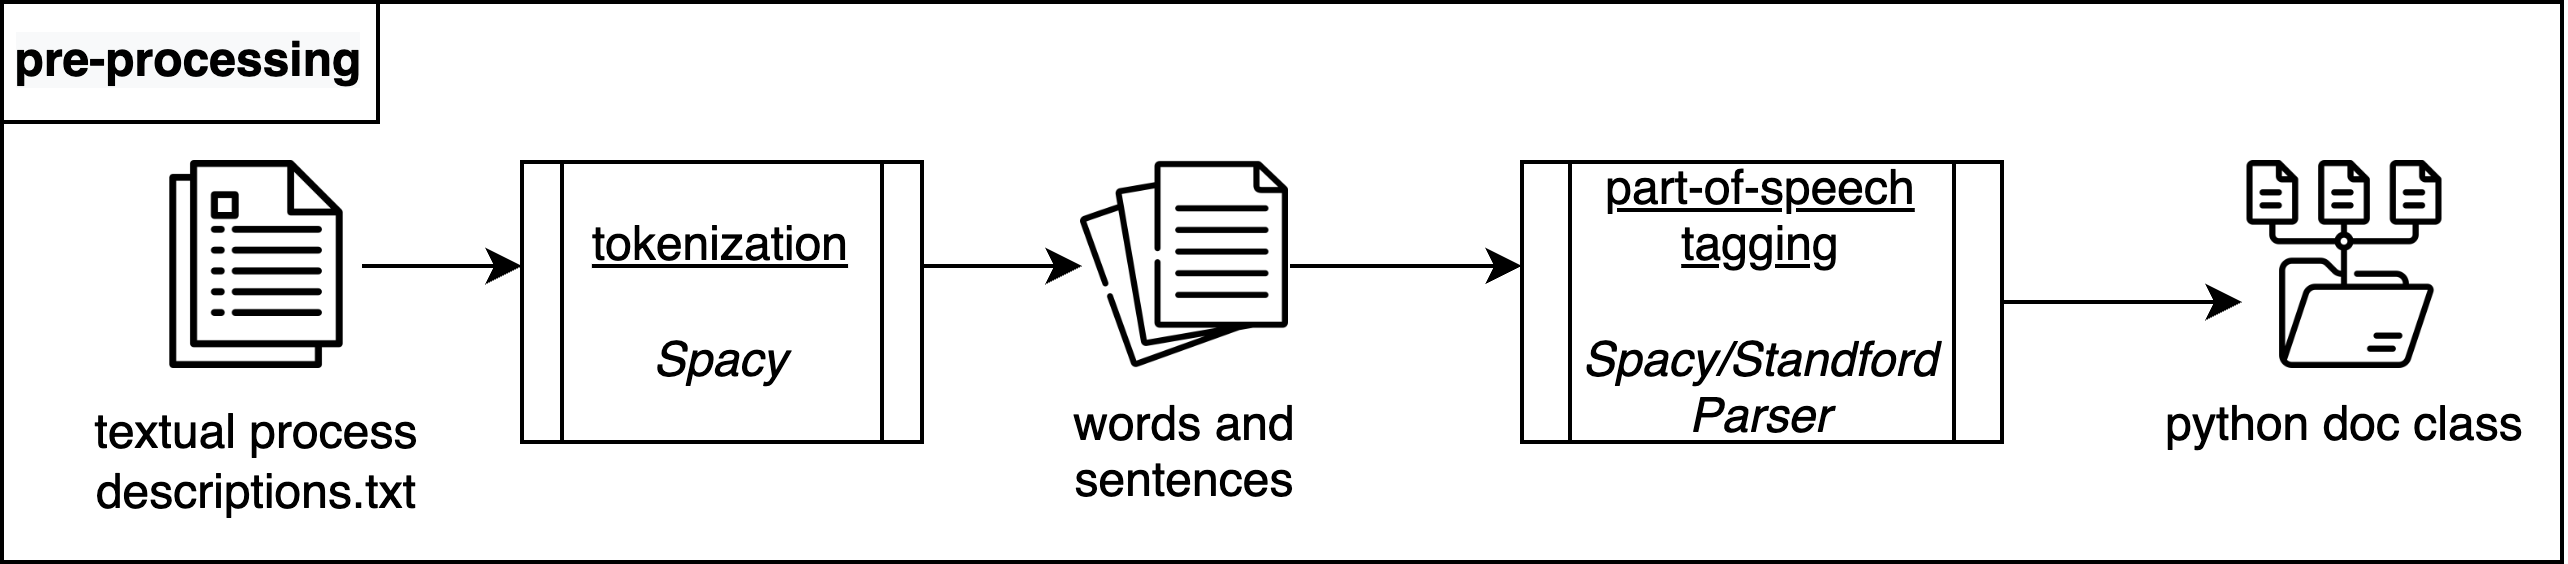
\includegraphics[width=0.8\textwidth]{tum-resources/images/theoretical_extraction_pre.png}
\end{figure}

The major step of information extraction is text-level analysis, where the sequential, conditional relationships of sentences will be exploited. In the central part of our work, we have to solve the anaphora resolution problem, which refers to the word that represents a word or a phrase that occurred beforehand \cite{literature_review_4}. Next, we have to solve the problem of finding conditional relationships between sentences. The conditional relationship is usually represented through a conditional word like "if", "else", "otherwise", etc. Finding these relationships is very crucial for the construction of logical conjunctions in the business model. Another essential task in the text-level analysis is the flow generation. A flow indicates how the business activities are related to each other and could be used to translate the processed information above into the business process model \cite{t2m_1}.

\begin{figure}[h]
    \centering
    \caption{Overview of processing}
    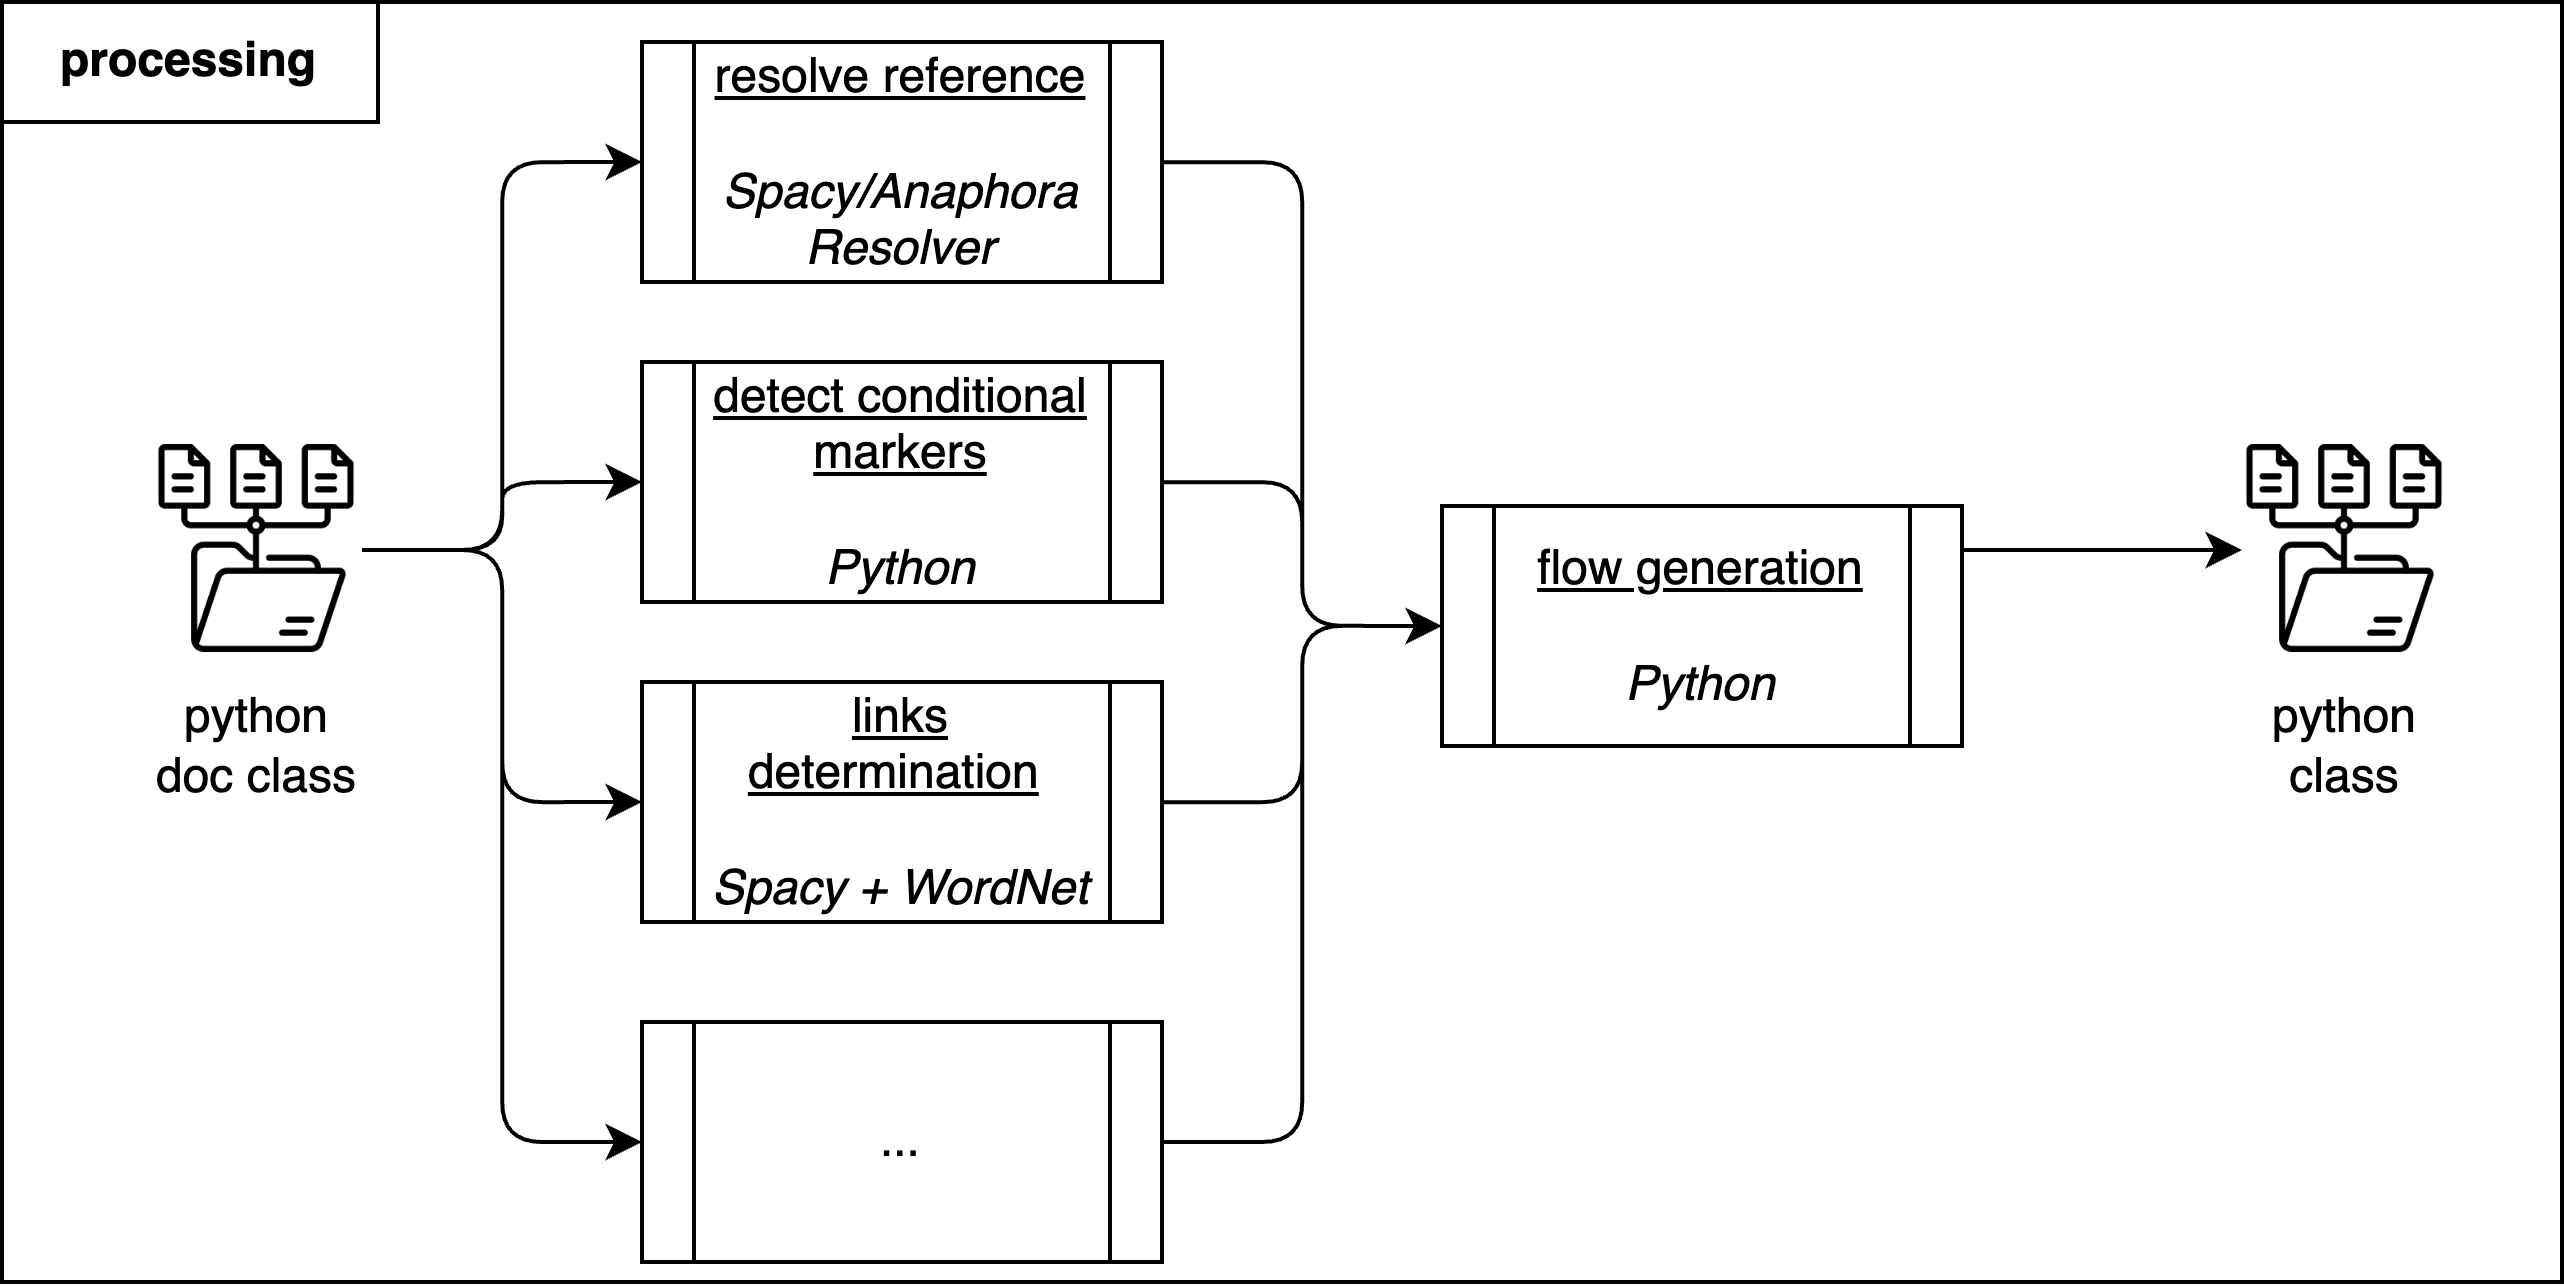
\includegraphics[width=0.8\textwidth]{tum-resources/images/theoretical_extraction_pro.png}
\end{figure}

After the flows of the model are generated, we could now perform the post-processing phase. Post-processing is about generating BPMN representation using the information acquired in the last two steps. \cite{t2m_1} suggests four steps of model generation: nodes creation, sequence flows construction, dummy elements removal, and open ends finishing. The nodes and edges will be created first to create the BPMN model. Then the dummy actions will be skipped, which are used to insert between gateways. Finally, the Start and the End events are to be created. \cite{complement_1} illustrate us to additionally implement a web interface that eases to use of the regulatory document to BPMN model transmission service. The web interface should take the text description as input and then will represent the BPMN model in the webpage after the text is processed with our model in the backend.

\begin{figure}[h]
    \centering
    \caption{Overview of post-processing}
    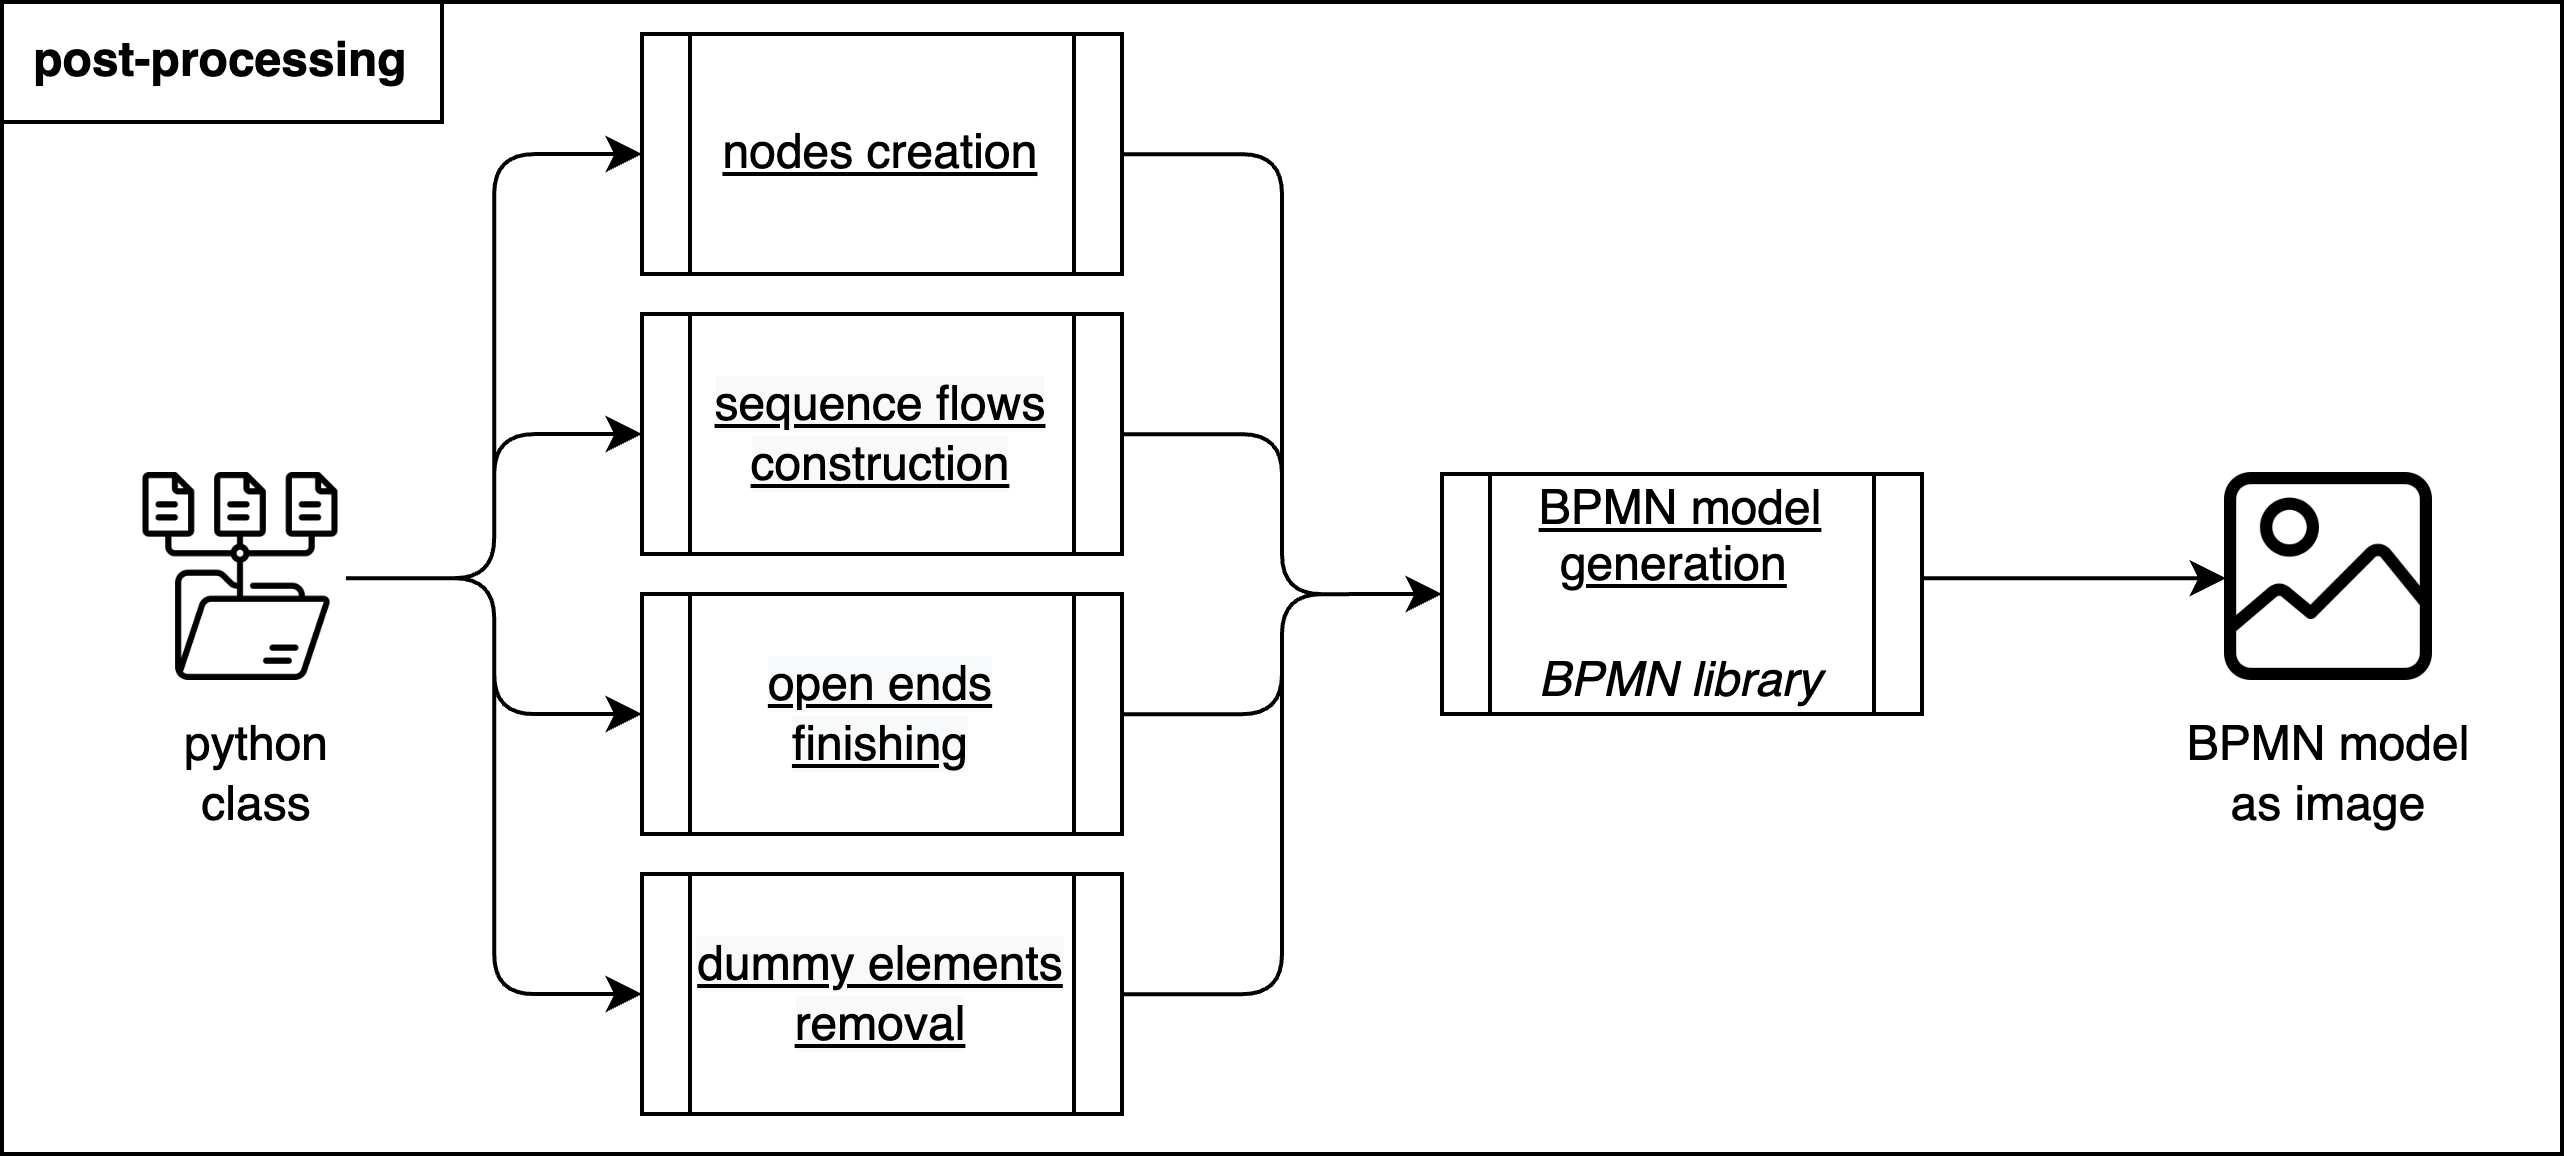
\includegraphics[width=0.8\textwidth]{tum-resources/images/theoretical_extraction_post.png}
\end{figure}
